\DiaryEntry{Single-Source Shortest Paths}{2020-04-02}{Algorithms}

\subsection{Introduction}

We are given a weighted, directed graph $G=(V,E)$ with a weight function $w: E \rightarrow \mR$ mapping edges to real-valued weights. A path $p$ is a sequence of edges, $p=\langle v_0,v_,\cdots,v_n \rangle$; its \emph{weight} $w(p)$ is given by the sum of its edges

\bee
w(p) = \sum_{i=1}^n w(v_{i-1},v_i)
\eee

The \emph{shortest-path weight} $\delta(u,v)$ from vertex $u$ to vertex $v$ is defined as

\bee
\delta(u,v) = \begin{cases} \min_p w(p): u \rightarrow v \, & \text{if there is a path from u to v} \\ \infty \, & \text{otherwise} \end{cases}
\eee

A \emph{shortest path} from $u$ to $v$ is then any path from $u$ to $v$ with weight $w(p) = \delta(p)$. There can be more than one shortest path between $u$ and $v$.

In this entry, we focus on \emph{single-source shortest paths problems}; i.e. we are given one source egde $s \in V$ and determine shortest paths to all vertices $v \in V$. 

The followig theorem helps in  with finding shortest paths.

\begin{theorem}
Given a weighted graph $G=(V,E)$ with weight function $w: E \rightarrow \mR$, let $p=\langle v_0,v_,\cdots,v_n \rangle$; be a shortest path from vertex $v_0$ to vertex $v_n$, and, for any $i$ and $j$ such that $0 \leq i \leq j \leq n$, let $p_{ij} = \langle v_i,v_,\cdots,v_j \rangle$ be the subpath of $p$ from vertex $v_i$ to vertex $v_j$. Then, $p_{ij}$ is a shortest path from $i$ to $j$. 
\end{theorem}

\begin{proof}
If we decompose the path $p$ into $v_0 \overset{p_{0i}}{\sim} v_i \overset{p_{ij}}{\sim} v_j \overset{p_{jk}}{\sim v_k}$, then we have $w(p) = w(p_{0i}) + w(p_{ij}) + w(p_{jk})$; i.e. the weights are additive. Now, assume that there is a path $p'_{ij}$ from $v_i$ to $v_j$ with weight $w(p'_{ij}) < w(p_{ij})$. Then, we can decompose $p$ also into $v_0 \overset{p_{0i}}{\sim} v_i \overset{p'_{ij}}{\sim} v_j \overset{p_{jk}}{\sim v_k}$ whose weight is $w(p_{0i}) + w(p'_{ij}) + w(p_{jk}) < w(p)$. However, this contradicts the assumption that $p$ is a shortest path from $v_0$ to $v_k$.
\end{proof}

While this theorem may seem trivial, it is imporant as it ensures that the single-source shortest path problems are unique. In particular, when $i=0$ and $0 \leq j \leq n$, we have subpaths of the form $p_{0j} = \langle v_0,v_,\cdots,v_j \rangle$ which are the shortest paths between $v_0$ and $v_j$. This implies that single-source shortest path algorithms return a tree. This tree can be described by each vertex having a predecessor attribute.   

In the following example graph, assume that $\langle v_0, v_1, v_2, v_3 \rangle$ is a shortest path between $v_0$ and $v_3$ and  $\langle v_0, v_p, v_2, v_3 \rangle$ is \emph{not} a shortest path. Then the shortest path between $v_0$ and $v_2$ is the path $\langle v_0, v_1, v_2 \rangle$.

\begin{figure}[H]v
\centering
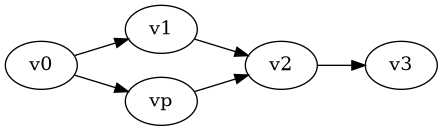
\includegraphics[scale=0.5]{images/sssp_0.png}
\end{figure}

If the path $\langle v_0, v_p, v_2 \rangle$ would be the shortest between $v_0$ and $v_2$, single-source shortest path algorithms would not return a tree and the predecessor attribute would not be enough / path-dependent.


\paragraph{Example.} We consider the following weighted graph as example.


\begin{figure}[H]
\centering
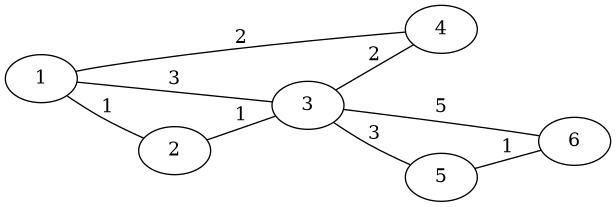
\includegraphics[scale=0.5]{images/sssp_1.png}
\end{figure}


If we choose the source vertex $s=1$ and run a single-source shortest path algorithm (Bellman-Ford), we obtain the following result: The algorithm returns a tree (via a predecessor graph) which is shown in red in the Figure below.


\begin{figure}[H]
\centering
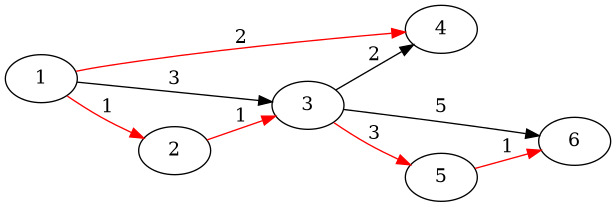
\includegraphics[scale=0.5]{images/sssp_2.png}
\end{figure}

In addition, the algorithm provides the distance between the source and each vertex. This is shown in the Table below.

\begin{tabular}{c|c}
  Vertex & Distance \\ \hline
  1 & 0 \\
  2 & 1 \\
  3 & 2 \\
  4 & 2 \\
  5 & 5 \\
  6 & 6
\end{tabular}

\paragraph{Negative Weights and Cycles.} Some algorithms allow for negative edge weights. A necessary condition for a soluton is, that there are no cycles with negative weights: If there would be, then no path can be shortest (minimum weight) as appending (another) cycle to a path would create a path with even lower weight. An example of this is shown in the following Figure: There is a cycle of negative weight $-3$ between vertices $2$ and $3$. Any path between vertices $1$ and $4$ can be made shorter by running around this cylce one more time.

\begin{figure}[H]
\centering
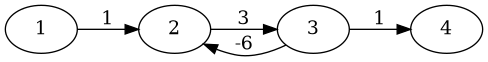
\includegraphics[scale=0.5]{images/sssp_3.png}
\end{figure}

From a general perspective, shortest paths cannot contain cycles:

\begin{itemize}
\item Cycle with negative weight are not allowed as there no shortest paths (see above).
\item Cycles with positive weight can be elimated and yield a shorter path.
\item Cycles with zero weight, do not affect the path weight, but cano be removed without changing the weight of the shortest path.
\end{itemize}


\paragraph{Relaxation.} 

For each vertex $v$ we maintain an attribute $v.d$ which is an upper bound of the weight of a shortest path from source $s$ to $v$. This attribute is called shortest-path estimate. In addition, for every vertex $v$ we have a predecessor $v.\pi$. The shortest path algorithms set this attribute accordingly; by starting at a vertex $v$ and ``tracing back'' to vertex $s$, we obtain the shortest path between $s$ and $v$.

These two attributes are initialzed as follows:

\begin{verbatim}
Init-Single-Source(G,s)
   for each vertex v in G
      v.d = INF
      v.pi = NULL
   s.d = 0
\end{verbatim}

Relaxing an edge $(u,v)$ means to test whether we can improve the shortest path to vertex $v$ found so far by going through vertex $u$. If this is the case, then we update $v.\pi$ and $v.d$.

The relaxation algorithm looks as follows

\begin{verbatim}
Relax(u,v,w)
   if v.d > u.d + w(u,v)
      v.d = u.d + w(u,v)
      v.pi = u 
\end{verbatim}

An example is shown in the following Figure. Left (a):  The upper bound is $v.d = 9$; if we choose going via vertex $u$ instead, we can tighten the bound to $v.d = u.d + w(u,v) = 5 + 2 = 7$. In the right Subfigure (b), this is not possible; going via vertex $u$ instead, would increase $v.d$ and therefore relaxation is not possible.   


\begin{figure}[H]
\centering
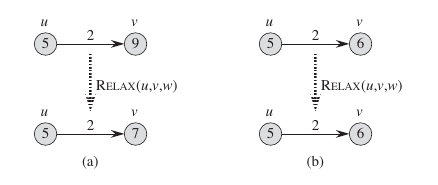
\includegraphics[scale=0.65]{images/sssp_4.png}
\end{figure}



\subsection{Bellman-Ford Algorithm}

The Bellman-Ford algorithm looks as follows.


\begin{Verbatim}[numbers=left, xleftmargin=5mm]
Bellman-Ford(G, w, s)
   Init-Single-Source(G,s)
   for i = 1 to |G.V|-1
      for each edge (u,v) in G.E
         Relax(u,v,w)
   for each edge (u,v) in G.E
      if v.d > u.d + w(u,v)
         return false
   return true
\end{Verbatim}

After initializing all vertices (line $2$), the algorithm runs $|G.V|-1$ times across all edges (lines $3$ and $4$). For each edge, it performs a relaxation (lines $5$). After that it is finished; it remains to chekc whether there are any negative cycles. This is achieved by checking the condition in line $7$ for all edges; if the condition holds for one edge, there is a cycle of negative weight and the algorithm terminates.


\paragraph{Example.} We consider the following mini-example to illustrate how the algorithm works.

\begin{figure}[H]
\centering
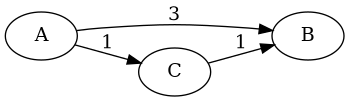
\includegraphics[scale=0.5]{images/sssp_5.png}
\end{figure}

For the illustration, we write inside the vertices the values of \verb d and \verb pi . We choose \verb s=A and after running \verb Init-Single-Source(G,s) , we have the following values.

\begin{figure}[H]
\centering
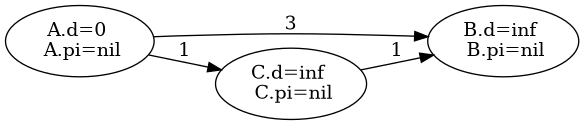
\includegraphics[scale=0.5]{images/sssp_6.png}
\end{figure}

The algorithm will now run $|G.V|-1 = 2$ times over all edges and perform relaxation. The order in which the algorithm chooses the edges is arbitrary. Depending on the order, the algorithm may finish earlier; i.e. no updates occur in later iterations.

We first start with the edge \verb A-B . Relaxation is possible; i.e. \verb B.d>A.d+w(A,B) . Therefore, we set \verb B.d=3  and \verb B.pi=A . This results in the following attributes of the graph.

\begin{figure}[H]
\centering
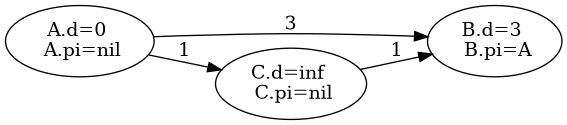
\includegraphics[scale=0.5]{images/sssp_7.png}
\end{figure}

Next we choose the edge \verb A-C . Again, relaxation is possible and we set \verb C.d=1  and \verb C.pi=A . We get the following graph.

\begin{figure}[H]
\centering
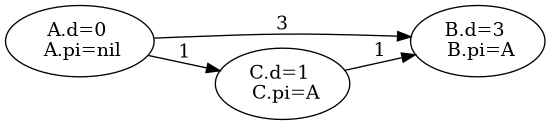
\includegraphics[scale=0.5]{images/sssp_8.png}
\end{figure}

There is the edge \verb B-C left. Again, we can relax and update \verb B.d=2  and \verb B.pi=C . We finally arrive at the graph as follows.

\begin{figure}[H]
\centering
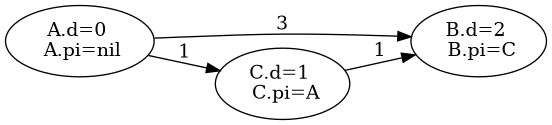
\includegraphics[scale=0.5]{images/sssp_9.png}
\end{figure}

We have chosen the edges in the ``right'' order and already obtained the final solution after the first iteration. We have one more iteration ``left''; however, this won't change anything.

\paragraph{Example - Negative-weight Cycle} Now let's consider a graph with a negative-weight cycle. 

\begin{figure}[H]
\centering
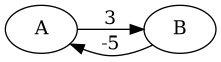
\includegraphics[scale=0.5]{images/sssp_15.png}
\end{figure}

After running \verb Init-Single-Source(G,s) , we have the following values.

\begin{figure}[H]
\centering
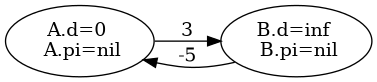
\includegraphics[scale=0.5]{images/sssp_16.png}
\end{figure}

We start with the edge \verb A-B . We perform relaxation and arrive at

\begin{figure}[H]
\centering
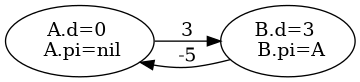
\includegraphics[scale=0.5]{images/sssp_17.png}
\end{figure}

Next we consider the egde \verb B-A . Contrary to the previous example, we also perform relaxation and arrive at the following

\begin{figure}[H]
\centering
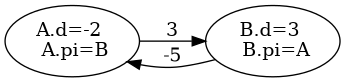
\includegraphics[scale=0.5]{images/sssp_18.png}
\end{figure}

Here the algorithm stops (we have $|G.V| -1 = 1$ iterations). However, if we would continue to run the algorithm, the values $A.d$ and $B.d$ do not stay constant but are getting less and less. This is the symptom of a negative-weight cycle.

The Bellman Ford algorithm performs a check for such negative-weight cycles. Looking at edge \verb A-B , we need to check whether $B.d \geq A.d + w(A,B)$: We have $3 \geq -2 + 3 = 1$, the condition is true and we return \verb false  to indicate a negative-weight cycle.


\subsection{Single-source Shortest Paths in DAGs}

The example from the previous Section indicates that for some graphs the full number of iterations in the Bellman-Ford algorithm is needed. This is inparticular the case of graphs without cycles; i.e. directed acyclic graphs (DAGs). When they are traversed in the ``right order'', one iteration of relaxation is sufficient. The right order is given by a topological sort of the vertices. Taken together, the complete algorithm for the single-source shortest path algorithm for DAGs is given as follows.

\begin{verbatim}
DAG-Shortest-Paths(G, w, s)
   topologically sort vertices G.V
   Init-Single-Source(G,s)
   for each vertex u taken in topological order
      for each vertex v in G.Adj[v]
         relax(u,v,w)
\end{verbatim}

The check for negative weight cycles can be omitted, as a DAG has no cycles.



%%% Local Variables:
%%% mode: latex
%%% TeX-master: "journal"
%%% End:
